%%%%%%%%%%%%%%%%%%%%%%%%%%%%%%%%%%%%%%%%%%%%%%%%%%%%%%%%%%%%%%%%%%%%%%%%%%%%%%%%
\documentclass[12pt]{article}

\usepackage[authoryear]{natbib}
\usepackage[top=2.5cm,bottom=2.5cm,left=2.5cm,right=2.5cm]{geometry}
\usepackage{color}
\usepackage{chemarr}
\usepackage{amssymb}
\usepackage{graphicx}
\usepackage{textcomp} 
\usepackage[gen]{eurosym}
\usepackage{amsmath}
\usepackage[margin=1.5cm]{caption}
\usepackage{amsmath,mathtools}
\usepackage{subcaption}
%\usepackage{ulem}
\usepackage[normalem]{ulem}
%\setlength{\belowcaptionskip}{-5pt}
%\setlength{\abovecaptionskip}{-8pt}
\usepackage{enumitem}
\usepackage{setspace}
\usepackage{nth}
\doublespacing

%\usepackage[autolinebreaks,useliterate]{mcode}
\usepackage[usenames, dvipsnames]{xcolor}
\colorlet{shadecolor}{gray!5}

\newcommand{\nrtodo}[1]{{\color{blue} NR: #1}}
%%%%%%%%%%%%%%%%%%%%%%%%%%%%%%%%%%%%%%%%%%%%%%%%%%%%%%%%%%%%%%%%%%%%%%%%%%%%%%%%
\title{\textbf{Thesis Draft}}
\author{Yinrui Li}
\date{}


%\maketitle


\begin{document}
	\maketitle
	%%%%%%%%%%%%%%%%%%%%%%%%%%%%%%%%%%%%%%%%%%%%%%%%%%%%%%%%%%%%%%%%%%%%%%%%%%%%%%%%
	
	
	
	\section{Introduction} 
	Black carbon (BC) is a product of incomplete combustion of fossil fuel, biofuel and biomass burning (Bond et al., 2004; Forsstrom et al., 2013). It strongly absorbs visible light and has been ranked as the 2nd most important individual absorbing agent after CO2, with a climate forcing of +1.1Wm-2 (Bond et al., 2013). Generally, BC aerosols can impact the global atmospheric radiative budget both as atmospheric aerosols, after mixing with other soluble organic materials, or as impurities in snow and ice after being transported to the polar regions and depositing onto their surfaces, resulting in a positive feedback on the surface albedo (Zuberi et al., 2005; Flanner et al., 2007). BC aerosols also have adverse impacts on air quality and human health (Highwood and Kinnersley, 2006).

	Quantifying these impacts requires us to develop faithful model representations of BC burden and its climate-relevant properties such as CCN activities and optical properties. Currently, however, significant discrepancies in model simulated BC remain in most global climate models (GCMs) and large uncertainties of its climate forcing have been shown. For example, previous studies have implied a general overestimation of BC in the mid-upper troposphere in the mid-latitudes, and an underestimation of BC in the lower and middle troposphere at high latitude (Koch et al., 2009; Schwarz et al., 2010; Fan et al., 2012). The simulated BC aerosol absorption optical depth tends to be biased low compared to satellite observations (Koch et al., 2009). These model failures can result from the complex BC aerosol processes and properties that has not been well captured, such as its emissions, coagulation, condensation, dry deposition, wet scavenging, etc. (Hakami et al., 2005; Koch et al., 2009; Shindell et al., 2008). These processes in turn control the evolution of aerosol burden, size distribution, mixing states, and consequently its climate forcing (Schulz et al., 2006; Quaas et al., 2009). 

	Among them, one key process that contributes to the uncertainties and thus needs to be captured is the BC ‘aging’ process, the conversion of freshly emitted, hydrophobic BC to aged, hydrophilic BC through coating with sulfate and organics or coagulation (Langner et al., 1992; Parungo et al., 1994; Liousse et al., 1996). This process directly contributes to the CCN activation and wet removal, and also impacts black carbon’s optical properties by evolving the composition and mixing states of aerosols. Therefore, it plays a significant role in simulating the lifetime of BC, and hence its transport, distributions and climate effects (Croft et al., 2005; Riemer et al., 2004). In addition, previous studies have found that the parameterizations of the aging process can significantly affect model results (Liu et al., 2011).

	Albeit its importance, the treatment of BC aging, however, is usually very simplified in global scale models, either by using fixed timescales or parameterized aging rates for the sake of computational limits. The most simplified bulk scheme assumes fully externally mixed populations and often use a fixed aging timescale (on the order of 1-2 days) for conversion of hydrophobic BC to hydrophilic BC (Cooke and Wilson, 1996). There are also more advanced and complicated schemes such as the modal aerosol model or sectional models, computing mechanic transfer rates by assuming aerosol size distributions and mixing levels (Wilson et al., 2001; Bauer et al., 2008, Huang et al., 2013). 

	The representation of BC aging in the Community Atmosphere Model with Chemistry (CAM-Chem), an atmospheric component of the Community Earth System Model (CESM), uses the latter scheme. It applies a 4-mode version of the modal aerosol model (MAM4), where BC is emitted to the primary carbon mode, and then is aged and transferred to the accumulation mode by condensation of sulfate, ammonia and SOA and by coagulation (Liu et al., 2012; Lamarque et al. 2012). In MAM4, a criterion of 8 monolayers of sulfate is used to compute the aerosol transfer rate from primary carbon mode to accumulation mode. It assumes that BC particle is aged after condensing 8 monolayers of sulfate. However, previous study has shown that considerable sensitivities exist regarding the choices of the number of monolayers and other parameters, and significant model biases in BC burden have been found compared to HIPPO observations (Liu et al., 2015). 

	Furthermore, Laura et al has derived a parameterization that characterizes the aging rates of BC aerosols through gas condensation and particle coagulation from detailed simulations on the particle scale, based on the particle-resolved PartMC-MOSAIC model (Particle Monte Carlo Model for Simulating Aerosol Inter- actions and Chemistry) (Laura et al., 2016). PartMC-MOSAIC is a complex aerosol model that provides detailed information on aging processes at the micro-scale, by tracing the size, composition and mixing states of particles (Riemer et al., 2010). That parameterization can be applied to evaluate and to improve the treatment of BC aging in the global-scale models. 

	In this work, our aim is to assess the representation of BC aerosols in MAM4 of CAMChem model. We conduct several sensitivity runs of BC mixing ratio, mixing states and direct radiative forcing to its condensation criterion, in order to investigate the extent to which those quantities are sensitive to the choices of aging parameters. We also exploit the PartMC-MOSAIC parameterization as the reference to evaluate the performance of MAM4 aging scheme. 

	Our method and model specification are described in Sect.2. Sensitivity analysis of BC is presented in Sect.3. In Sect.4, we focus on process analysis of BC aging by comparing the CAMChem aging timescales with PartMC aging timescales. In Sect.5, we assess the comparability of modeled BC concentration with SP2 measurements. The results are shown in Sect.6. 

	\section{Background}
	
	\subsection{Modal Aerosol Model}
	\subsubsection{Aerosol Dynamic Modeling}
	Aerosols have complex physical processes and a numerical aerosol model can serve as an useful tool to extend our knowledges of aerosol evolution in the atmosphere. Generally, an aerosol model should be able to assemble expressions for the relevant physical processes including coagulation, condensation, nucleation, emission, chemical reaction, etc (Whitby et al., 1991). The approaches to solve those expressions differ by the way that aerosol size distributions are approximated. Some traditional models characterize the particle size distribution as bulk or by single variable such as mass. More complicated models include sectional model that sets discrete size bins and typically assumes species to be internally mixed in each bins and externally mixed between different bins (Jacobson et al., 1997, Adams et al., 1999). This approach neglects the aging process by assuming particles to be internally mixed immediately after emission. Another frequently used representation is called the modal aerosol model (Whitby et al., 1992; Binkowski et al., 1995). Aerosols are viewed as distinct populations of particles that is distinguished by their size or chemical composition, and the size distribution of each population is approximated by some analytical distribution function (Binkowski et al., 1995). Each region of the size distribution is called a mode. The size of the particles in each population is typically approximated by a lognormal distribution characterized by the mean diameter $\mu$ and a standard deviation $\sigma$. The accuracy of the model largely depend on how well the size distribution functions of the modes can represent the actual aerosol size distributions.  
	
	Figure~\ref{fig_P4} shows a typical categorization of aerosols by their size distributions. Particles less than 0.1~$\mu$m go into the nucleation mode, particles in the size range 0.1--2~$\mu$m go into the accumulation mode, and particles larger than 2~$\mu$m go into the coarse mode. Similarly, in CAM-chem model, a 3-mode version of modal aerosol model (MAM3) that has only Aitken, accumulation and coarse mode is developed as default, which is efficient for long-term simulations (Liu et al., 2012). There are also a 7-mode version (MAM7) that has Aitken, accumulation, primary carbon, fine dust and fine sea salt, coarse dust and coarse sea salt modes, and a 4-mode version (MAM4) that has an additional primary carbon mode on top of MAM3 for the treatment of the microphysical aging processes of primary carbonaceous aerosols (Liu et al., 2015). 
	\begin{figure}[!h] 
		\begin{center}
			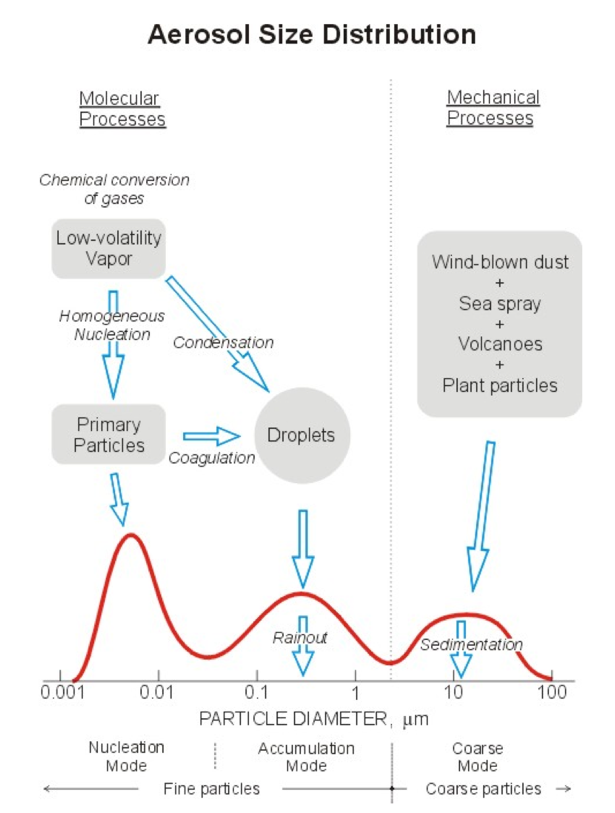
\includegraphics[width = 0.6\textwidth]{Figure04}
			\caption[]{\label{fig_P4} Aerosol Size Distribution. (www.ems.psu.edu/~lno/Meteo437)}
		\end{center}
	\end{figure}
		
	\subsubsection{Moment and Moment Dynamic Equation}
	Modal aerosol model typically assumes lognormal size distributions for each mode (Equation ~\ref{eq:1}) by setting an changeable mean diameter $D_{\rm g}$ and an unchangeable standard deviation $\sigma_{\rm g}$. 
	\begin{align}\label{eq:1}
	n(\text{ln}D) = \frac{N}{\sqrt{\pi}\text{ln}\sigma_{\rm g}}\text{exp}[-\frac{1}{2}(\frac{\text{ln}(D/D_{\rm g})}{\text{ln}\sigma_{\rm g}})^2]
	\end{align}
	During each time step, it simulates the evolution of aerosols by updating the geometric mean diameter $D_{\rm g}$, total number concentration $N$ and standard deviation $\sigma_{\rm g}$ for each mode, solved from their aerosol dynamic differential equations. Those differential equations are designed to catch the physical processes that will drive the evolution of aerosols, such as coagulation, condensation, nucleation, emission, chemical reaction, etc.
	
	 However, while the differential equations for the total number $N$ is easy to obtain, it is hard to find the analogous equations for $D_{\rm g}$ and $\sigma_{\rm g}$. In order to avoid this problem, some kind of integral form called moment is hence introduced to replace the traditional form of differential equations. The mathematical expression of the kth moment is defined as:
	 \begin{align}
	 M_\text{k} = \int_{-\infty}^{+\infty}D^kn(\text{ln}D)d\text{ln}D = ND_{\rm g}^k\text{exp}[\frac{k^2}{2}\text{ln}^2\sigma_{\rm g}]
	 \end{align}
	 \begin{flushleft}
	 	$k = 0$ : total number $N = M_0$ \\
	 	$k = 2$ : total surface area $S = \pi M_2$ \\
	 	$k = 3$ : total volume $V = \frac{\pi}{6}M_3$ \\
	 \end{flushleft}
	, where the total number, surface area and volume of particles in one mode are analogous to the \nth{1} moment, \nth{2} moment and \nth{3} moment respectively. 
	
	The corresponding integral form of dynamic differential equation, called moment dynamic equation, is shown below (Binkowski et al., 1995):
	\begin{figure}[!h]
		\begin{center}
			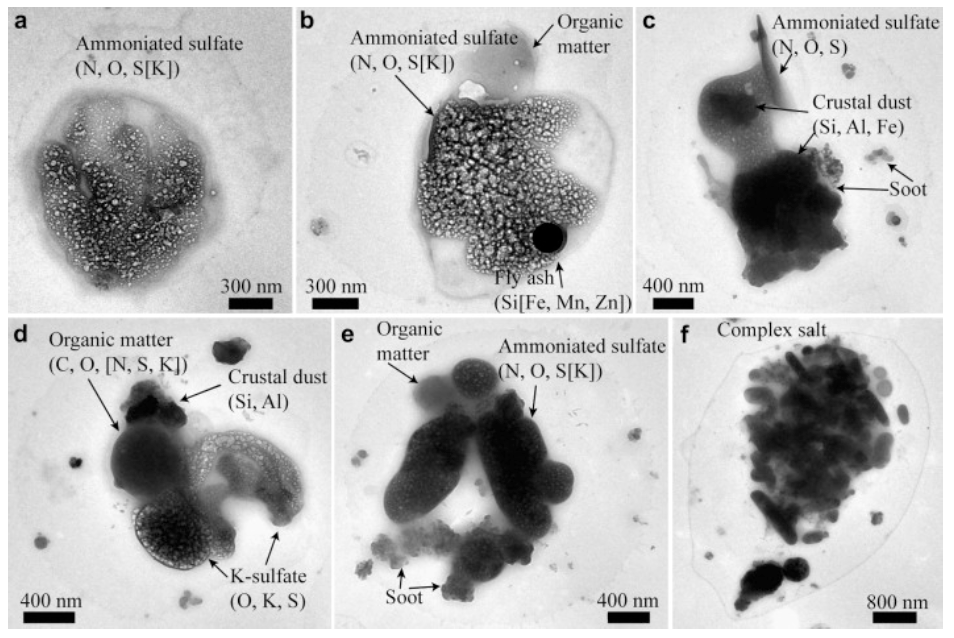
\includegraphics[width = 0.9\textwidth]{Figure05}
		\end{center}
	\end{figure}
	
	
	
	\newpage
	Generally, modal aerosol model will solve the moment differential equations for $M_0$, $M_3$ and $M_6$, and then derive $N$, $D_{\rm g}$ and $\sigma_{\rm g}$ from the three moments. $M_6$ is chosen because the coagulation term can be integrated analytically. 
	
	In our study, we used a 4-mode version of modal aerosol model (MAM4) of CAM-chem that has aitken mode, accumulation mode, coarse mode and a specially designed primary carbon mode for the treatment of the microphysical aging processes of primary carbonaceous aerosols. More description about MAM4 is in section 3.1. MAM4 assumes that the standard deviation $\sigma_{\rm g}$ for each mode is fixed, whereas $N$ and $D_{\rm g}$ are changeable with time. For each time step the model will solve the dynamic differential equations for $M_0$ and $M_3$, and then derive $N$ and $D_{\rm g}$ from the two moment equations.
	
	\subsection{Mixing States and its Impact on Climate}
	
	\subsection{BC Mixing States in the Arctic}
	
	\subsection{Size Range of SP2 Measurement}
		The SP2 instrument measures the BC particle cores over a calibrated volume equivalent diameter (VED) range of 55--400~nm, which is unlikely to represent the total
		ambient number and mass concentrations of BC particles (Reddington et al., 2013). In order to compare CAMChem model simulated BC with observations, we estimated the mass fraction of modeled BC in the size range corresponding to SP2 measurement. SP2 number-detection efficiency at sea level pressure is reported to be 100$\%$ for BC above 90~nm VED (Schwarz et al., 2010a), so following Reddington et al., 2013, we use 90~nm--400~nm as the efficient diameter range of SP2 measurement in this study.
	
	\section{Methodology}

		\subsection{CAM-chem Model Configurations and MAM4}
		
		CAM-chem model is a global 3-D atmospheric component of the NCAR Community Earth System Model (CESM). It consists of the Community Atmosphere Model (CAM) model and chemical mechanism of a fully implemented model for ozone and related chemical tracers (MOZART-4) which includes 191 chemical tracers and over 400 reactions (Tilmes et al., 2016). CAM-chem model can be run either with interactive meteorology coupled to a free-running ocean with specified sea ice and sea surface temperature (free-running configuration), or with specified meteorology which read in winds, air temperature, surface pressure and heat fluxes (offline configuration) (Lamarque et al., 2012). It is also coupled to the land model, involving emissions from biogenic sources by the Model of Emissions and Aerosols from Nature (MEGAN) (Guenther et al., 2012). 

		For our study, we chose the CESM 1-2-2 CAM-chem configured with the offline meteorological data from the Global Earth Observing System (GEOS-5) of the Global Modeling Assimilation Office of NASA, and launched one-year simulation for 2010 with a standard horizontal resolution of 1.9  latitude by 2.5 longitude and a vertical resolution of 56 layers in order to match the resolution of the input meteorology field. We use the Intergovernmental Panel on Climate Change (IPCC) Fifth Assessment report (AR5) gridded POM and BC emissions for the period 1850-2010 in decadal increments (Lamarque et al., 2010). This inventory covers a wide range of sources including anthropogenic emissions (without injection heights) originating from domestic, energy, industry, transportation, waste treatment and ship activity sectors, and natural emissions (elevated) from forest fire and grass fire. It assumes that the POM emissions are higher than the OC emissions by a factor of 1.4 (Liu et al., 2012) and the injection heights for fires are from Dentener et al., 2006. The model treats hydrophobic BC and hydrophilic BC as two separate species, and all the freshly emitted BC falls into the first category. 

		There are three versions of modal representation of aerosol in CAM-chem. A 3-mode version of modal aerosol model (MAM3) that has only Aitken, accumulation and coarse mode is developed as default, which is efficient for long-term simulations (Liu et al., 2012). There are also a 7-mode version (MAM7) that has Aitken, accumulation, primary carbon, fine dust and fine sea salt, coarse dust and coarse sea salt modes, and a 4-mode version (MAM4) that has an additional primary carbon mode on top of MAM3 for the treatment of the microphysical aging processes of primary carbonaceous aerosols (Liu et al., 2015). MAM assumes lognormal size distributions for each mode by setting an unchangeable standard deviation and a changeable mean diameter, and predicts the changes of the size distributions of its particles with time in each mode. In MAM3, all BC particles are assumed to be aged and put directly into the accumulation mode, where particles are exposed to in-cloud and below-cloud wet deposition. In our study, we applied the newly developed MAM4 model, where the freshly emitted BC/POM particles will come directly into the hydrophobic primary carbon mode. The hygroscopicity of BC is set to be 0, and the hygroscopicity of POM is set to be 0.10, allowing them to experience some in-cloud scavenging in the primary carbon mode. After the aging process due to condensation of sulfate aerosols, ammonia and some semi-volatile organic aerosols and inter-mode or intra-mode coagulation, the fresh carbonaceous particles can be transferred from the primary carbon mode to the accumulation mode, viewed as being aged. A schematic of aerosol modes and associated tracers in MAM4 is shown in Figure~\ref{fig_P1}.
		\begin{figure}[!h] 
			\begin{center}
				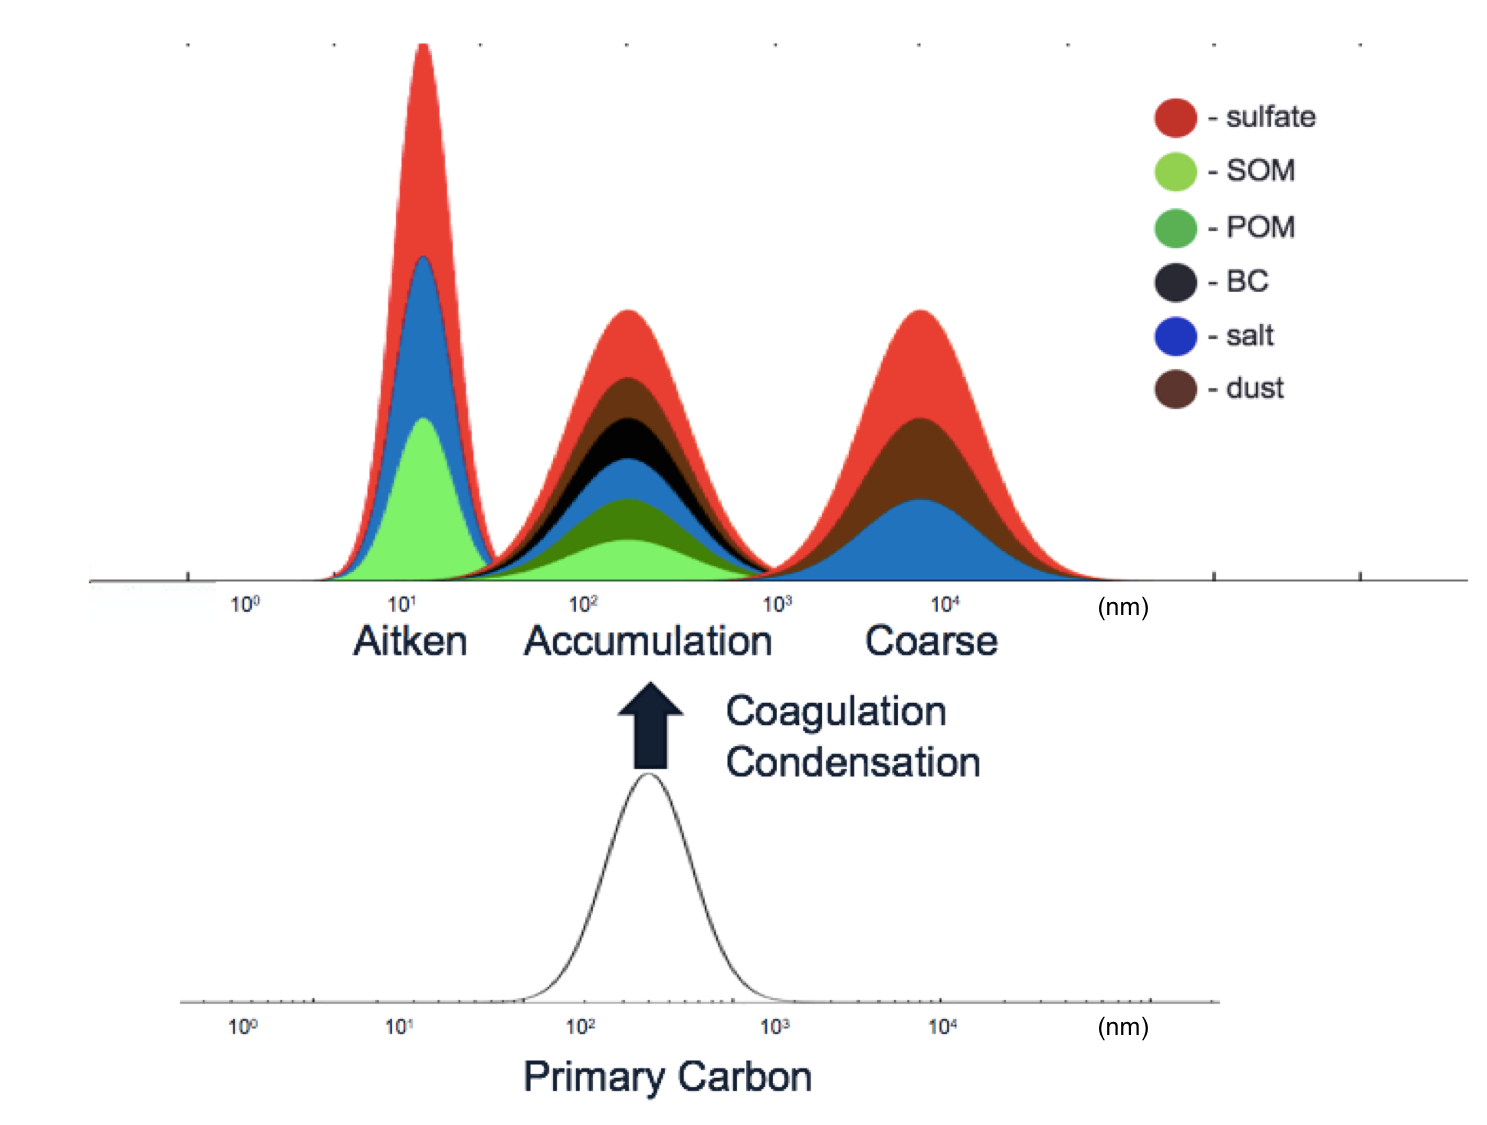
\includegraphics[width = 0.9\textwidth]{Figure01}
				\caption[]{\label{fig_P1} Schematic of aerosol modes and associated tracers in MAM4.}
			\end{center}
		\end{figure}
			
		
		 \subsection{8-monolayer of sulfate Condensation Criterion}
		
		 In MAM4, condensation of sulfate, ammonia and semi-volatile organics to carbonaceous particles are treated in a dynamic way, where a monolayer condensation criterion is applied. It assumes that BC particles become hydrophilic after condensing 8-monolayer of sulfate onto its core surface, and then this mass will be transferred from the primary carbon mode to the accumulation mode based on the standard mass transfer expressions, regarded as being aged (Liu et al., 2012). A schematic of the 8-monolayer condensation criterion is shown in Figure~\ref{fig_P3}. The depth of one monolayer of sulfate is equal to the molecular diameter of sulfate particle ($4.76\times 10^{-10}$~m).
		 \begin{figure}[!h] 
		 	\begin{center}
		 		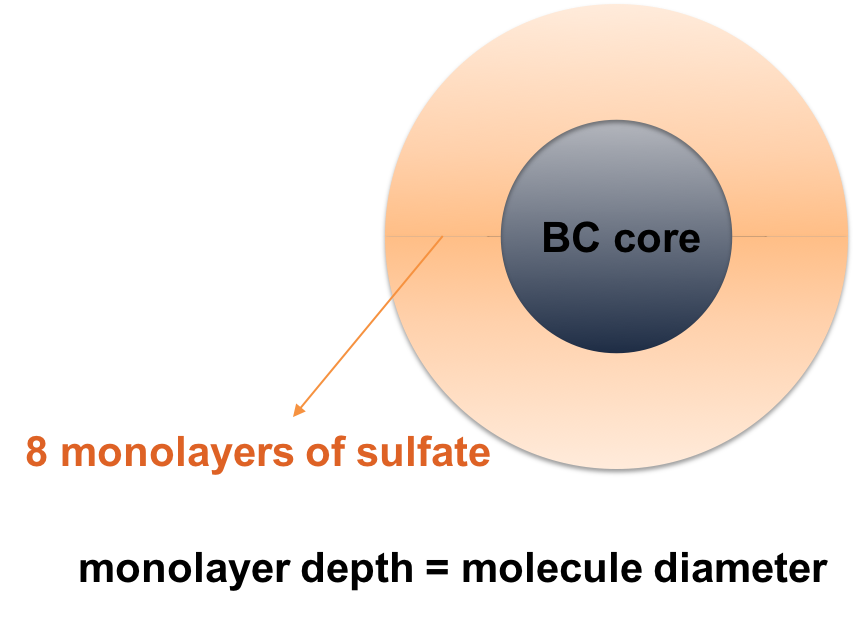
\includegraphics[width = 0.5\textwidth]{Figure03}
		 		\caption[]{\label{fig_P3} Schematic of 8-monolayer of sulfate criterion.}
		 	\end{center}
		 \end{figure}
		 
		 Currently, the condensation of sulfate and ammonia is assumed to be irreversible, whereas the condensation of semi-volatile organics (SOA) is reversible. Sulfate is produced from $\rm{SO}_{2}$ aqueous oxidation in bulk cloud water by ozone and $\rm{H}_{2}\rm{O}_{2}$, based on MOZART treatment (Tie et al., 2001). An accommodation coefficient (0.65), that is the probability of sticking when the gas molecules encounters the surface of an aerosol particle is used for all the three species (Liu et al., 2012). 
		 
		 Generally, for each time-step, the model computes the ratio of the  condensed soluble species mass in the primary carbon to the mass that is required to age all the particles in that mode based on the monolayer criterion. Then it assumes that the same ratio of the POM and BC in the primary carbon mode is transfered to the accumulation mode together with the condensed materials. Here we provide a detailed mathematical explanations of this model representation of the condensation scheme. 
		 
		 For each mode, the rate of gas uptake $F_\text{n}$ ($s^{-1}$) is represented as:
		 \begin{equation}
		 F_\text{n} = \int n(\text{ln}D_{\rm{p}})\times C d(\text{ln}D_\text{p}) ,
		 \end{equation}
		 where $D_\text{p}$ is the diameter of the aerosol particles in that mode, $n(lnD_\text{p})$ is the lognormal size distribution, and $C$ is the gas condensation rate (taking sulfuric acit for example):
		 \begin{align}
		 C = 2\pi \times D_\text{p} \times V_{\rm{diff}} \times F(K_\text{n}, A)  
		 \end{align}
		 
		 \begin{flushleft}
		 	$K_\text{n}$ : Knudsen number \\
		 	$A$ : accommodation coefficient \\
		 	$F$ : Fuchs-Sutugin correction factor \\
		 	$V_{\rm{diff}}$ : gas diffusivity for  $\rm{H_2SO_4}$
		 \end{flushleft}
		 The rate of total gas uptake $F_{\rm{sum}}$ is hence estimated by summing up $F_\text{n}$ over all 4 modes, and the fraction of gas mixing ratio going to each mode $f_\text{n}$ is equivalent to the ratio of $F_\text{n}$ to $F_{\rm{sum}}$.
		 \begin{align}
		 F_{\rm{sum}}  &= \sum_{k=1}^4 F_\text{n}          &
		 f_\text{n}          &= \frac{F_\text{n}}{F_{\rm{sum}}} 
		 \end{align}
		 
		 With the above information, the fraction of soluble species condensing on aerosols during $\Delta t$ is derived as $(1 - e^{-\Delta t\times F_{\rm{sum}}})$, and the mass mixing ratio of gas uptake that actually going to mode n during one time-step $\Delta t$ is:
		 \begin{equation}
		 \Delta q_\text{n} = q \times f_\text{n} \times (1 - e^{-\Delta t\times F_ {\rm{sum}}})
		 \end{equation}
	
		 The model computes the fraction of carbonaceous aerosols being aged $f_{\rm{age}}$ as the ratio of the volume of actually condensed materials $V_\text{shell}$ to the volume of soluble species required to age all the particles in the primary carbon mode $V_{\rm{8-mono}}$:
		 \begin{align}
		 \begin{split}
		 V_{\rm{shell}} &=  \Delta q_{\rm{SO_4}, n_{\rm{pc}}} \times V_{\rm{SO_4}} \\
		 &+ \Delta q_{\rm{NH_4}, n_{\rm{pc}}} \times V_{\rm{NH_4}} \\
		 &+ \Delta q_{\rm{SOA}, n_{\rm{pc}}} \times V_{\rm{SOA}} 
		 \end{split}
		 \end{align}
		 
		 \begin{align}
		 \begin{split}
		 V_{\rm{8-mono}} = (\pi M_2/ \frac{\pi}{6}M_3) \times d_{\rm{8-mono}}
		 \end{split}
		 \end{align}
		 
		 \begin{align}
		 f_{\rm{age}} &= \frac{V_{\rm{shell}}}{V_{\rm{8-mono}}}  
		 \end{align}
		 
		 \begin{flushleft}
		 	$V_{\rm{SO_4}}$, $V_{\rm{NH_4}}$, $V_{\rm{SOA}}$: factors that convert the unit of mixing ratio to $m^3/$kmol air. \\
		 	$V_{\rm{8-mono}}$: the volume of sulfate required to age all BC particles. \\
		 	$V_{\rm{core}}$: the volume of pure BC. \\
		 	$M_2$ $M_3$: second and third moment of  moment dynamic equation, $\pi M_2/ \frac{\pi}{6}M_3$ is the ratio of aerosol surface area to volume. \\
		 	$d_{\rm{8-mono}}$: the thickness of 8 monolayers of sulfate.
		 \end{flushleft}
		 
		 \subsection{CAM-chem Aging Timescale}
		 In a first-order aging model, the transition of BC mass from fresh to aged mode can be represented by an aging timescale. The model is given by
		 \begin{align}
		 \frac{dM_{\rm{fresh}}}{dt} = -\frac{1}{t_{\rm{aging}}}M_{\rm{fresh}} 
		 \end{align}
		 $M_{\rm{fresh}}$ is the mass of fresh particles.
		 The aging timescales can represented as the production of the inverse of the mass transfer rate and fresh BC mass. 
		 \begin{align}\label{eq:9}
		 t_{\rm{aging}} = M_{\rm{fresh}}/(-\frac{dM_{\rm{fresh}}}{dt})
		 \end{align}
		 Any particle transition from the fresh to aged mode during a time step is either by coagulation with other particles or by accumulating a certain amount of condensible materials. So the overall aging timescale $t_{\rm{aging}}$ can be represented as the combination of the aging timescales by condensation $t_{\rm{cond}}$ and by coagulation $t_{\rm{coag}}$.
		 \begin{align}\label{eq:10}
		 \frac{1}{t_{\rm{aging}}} =\frac{1}{t_{\rm{coag}}} + \frac{1}{t_{\rm{cond}}}
		 \end{align}
		 Each of the component aging timescales $t_{\rm{cond}}$ and $t_{\rm{coag}}$ can be derived from the corresponding mass transfer rate by applying Equation~ \ref{eq:9}. 
		 
		 In CAM-chem model, BC particles are transfered from the fresh, primary carbon model to the aged, accumulation mode according to mass transfer rates computed from the coagulation and condensation processes respectively. We extracted the mass transfer rates every 6 hours and apply Equation~\ref{eq:9} and Equation~\ref{eq:10} to get the corresponding timescales for aging. We would be able to evaluate the contribution of condensation and coagulation to the overall aging by showing their  timescales separately. In this study, we evaluated the monthly and annually averaged aging timescales. 
		 
		 \subsection{PartMC-MOSAIC Aging Timescale}
		 PartMC-MOSAIC (particle resolved model) can track the evolution of individual particles as they evolve through condensation, coagulation, emission and evaporation of SOA (Fierce et al., 2016). In current version of PartMC, the particles is not tracked individually but is instead assumed to be completely mixed. Previous study has investigated reduced representation of mixing state for simulating aerosol effects on climate (Fierce et al., 2016). It was discovered that using a detailed benchmarking model to simulate gas condensation and particle coagulation can represent simple mixing state sufficiently for modeling cloud condensation nuclei concentrations, and the mixing timescales that characterized this transformation have been parameterized. In our study, we applied that aging timescale parameterization to our global models outputs to evaluate the accuracy of our global model aging timescales.
		 
		Fierce et al applied a series of 100 sensitivity scenarios sampled using Latin hypercube sampling (McKay et al., 1979). Twenty-eight input parameters were applied to represent a range of atmospheric conditions, from highly polluted cases with consequently rapid aging to remote regions with slow aging. Those parameters include environmental variables, aerosol characteristics, aerosol type and gas emissions. In each scenario, they simulate the evolution of carbonaceous particles that is emitted into a population of background aerosol. No new fresh particle will be emitted during this process after the simulation starts, in order the isolate the effects of aging (Laura et al., 2016). The normalized error in the number concentration of CCN computed using the particle-resolved composition and the reduced representation of composition is given by:
		\begin{align}\label{eq:11}
		e_{\rm CCN}(t) = \frac{\int_{0}^{\infty}( \tilde{N}_{\rm CCN}(t,s) - 
			N_{\rm CCN} (t,s))ds}{\int_{0}^{\infty} \tilde{N}_{\rm CCN, q}(t,s)ds}
		\end{align}
		where $\tilde{N}_{\rm CCN}$ is the number concentration of CCN using the reduced composition and $N_{\rm CCN}$ is the CCN using the particle-resolved composition. This error decreases exponentially with time and a regression result has shown a high R-squared value as 93$\%$. The equation can be expressed as:
		\begin{align}
		e_{\rm CCN}(t) = e_{\rm CCN}(t_{0})\text{exp}(-\int_{t_{0}}^{t}\frac{1}{\tau_{\rm mix}(t)} dt) 
		\end{align}
		where $\tau_{\rm mix}$ is the overall aging timescale. 
		A particle is either aged by condensation or by coagulation, so the two processes can be treated as separate process and has their own timescale (Laura et al., 2015). Accordingly, the overall timescale is found to be a function of the condensation growth rate $I(t)$ and the particle number concentration $N(t)$.
		So a more specified parameterization of $\tau_{\rm mix}$ can be derived by regression of the error on $I(t)$ and $N(t)$:
		\begin{align}
		e_{\rm CCN}(t) = e_{\rm CCN}(t_{0})\text{exp}(-k_{\rm cond}\int_{t_{0}}^{t} I(t) dt)\text{exp}(-k_{\rm coag}\int_{t_{0}}^{t}N(t) dt) 
		\end{align}
		Figure~\ref{fig_P2} is an example of determining $k_{\rm coag}$ after setting $I(t)$ to be 0. 
		
		In our study, we computed the number concentration $N$ as the sum of the particle number concentration of all modes, and the condensation growth rate $I$ as the volume condensation rate over the total aerosol surface area. As is mentioned in 3.2, the condensation of SOA is reversible, so the total condensation rate can be positive or negative. Since all fresh BC particles are in the primary carbon mode, we computed the condensation growth rate using the volume condensation rate and surface area extracted from the primary carbon mode. The PartMC-MOSAIC parameterized aging timescales can then be represented as:
		\begin{align}
		\tau_{\rm overall} \approx (k_{\rm cond}I_{\rm cond} + k_{\rm coag}N)^{-1}
		\end{align}
		
		\begin{figure}[!h] 
			\begin{center}
				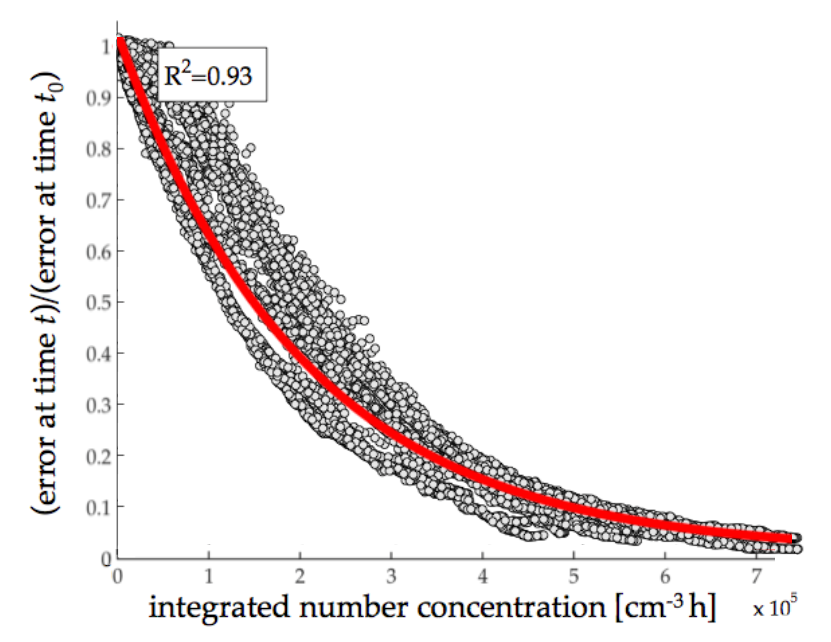
\includegraphics[width = 0.7\textwidth]{Figure02}
				\caption[]{\label{fig_P2}Raw data that is used to construct the regression function (grey dots) and the resulting regression function (black line) for simulations including only coagulation, without condensation (Fierce et al., 2016).}
			\end{center}
		\end{figure}
 
 	\clearpage
 	
	\section{Results}
	
	\subsection{Monolayers and Activation Ratio}

	
	
	
	
	
	
%	\bibliographystyle{plain-local-srefid}
%	\bibliography{refs}
	
	
	
	
	
	
	%%%%%%%%%%%%%%%%%%%%%%%%%%%%%%%%%%%%%%%%%%%%%%%%%%%%%%%%%%%%%%%%%%%%%%%%%%%%%%%%
	
References.

Bauer, S. E.,  S. Menon, D. Koch, T. C. Bond, and K. Tsigaridis. A global modeling study on carbonaceous aerosol microphysical characteristics and radiative forcing. Atmos. Chem. Phys., 10:4543–4592, 2010.

Bond, T. C., Streets, D. G., Yarber, K. F., Nelson, S. M., Woo, J. H.,and Klimont, Z.: A technology-based global inventory of black and organic carbon emissions from combustion, J. Geophys. Res.-Atmos., 109, D14203, doi:10.1029/2003jd003697, 2004.

Bond, T., Doherty, S., Fahey, D., Forster, P., Berntsen, T., DeAngelo, B., Flanner, M., Ghan, S.,Kärcher, B., and Koch, D.: Bounding the role of black carbon in the climate system: a scientific 10assessment, J. Geophys. Res.-Atmos., 118, 5380–5552, doi:10.1002/jgrd.50171, 2013.

Cooke, W. F., and J. N. Wilson. A global black carbon aerosol model. J. Geophys. Res., 101:19395–19408, 1996.
Croft, B., Lohmann, U., and von Salzen, K.: Black carbon ageing in the Canadian Centre for Climate modelling and analysis atmo- spheric general circulation model, Atmos. Chem. Phys., 5, 1931– 1949, doi:10.5194/acp-5-1931-2005, 2005. 
Liu, J. F., Fan, S. M., Horowitz, L. W., and Levy, H.: Evalua- tion of factors controlling long-range transport of black car- bon to the Arctic, J. Geophys. Res.-Atmos., 116, D04307, doi:10.1029/2010jd015145, 2011. 

Riemer, N., Vogel, H., and Vogel, B.: Soot aging time scales in polluted regions during day and night, Atmos. Chem. Phys., 4, 1885–1893, doi:10.5194/acp-4-1885-2004, 2004. 

Schwarz, J. P., Spackman, J. R., Gao, R. S., Watts, L. A., Stier, P., Schulz, M., Davis, S. M., Wofsy, S. C., and Fahey, D. W.: Global- scale black carbon profiles observed in the remote atmosphere and compared to models (vol 37, art L18812, 2010), Geophys. Res. Lett., 37, L23804, doi:10.1029/2010gl046007, 2010. 

Shindell, D. T., Chin, M., Dentener, F., Doherty, R. M., Faluvegi, G., Fiore, A. M., Hess, P., Koch, D. M., MacKenzie, I. A., Sander- son, M. G., Schultz, M. G., Schulz, M., Stevenson, D. S., Teich, H., Textor, C., Wild, O., Bergmann, D. J., Bey, I., Bian, H., Cuve- lier, C., Duncan, B. N., Folberth, G., Horowitz, L. W., Jonson, J., Kaminski, J. W., Marmer, E., Park, R., Pringle, K. J., Schroeder, S., Szopa, S., Takemura, T., Zeng, G., Keating, T. J., and Zu- ber, A.: A multi-model assessment of pollution transport to the Arctic, Atmos. Chem. Phys., 8, 5353–5372, doi:10.5194/acp-8- 5353-2008, 2008. 

Fan, S. M., Schwarz, J. P., Liu, J., Fahey, D. W., Ginoux,P., Horowitz, L. W., Levy, H., Ming, Y., and Spackman, J. R.: Inferring ice formation processes from global-scale black carbon profiles observed in the remote atmosphere and model simulations, J. Geophys. Res.-Atmos., 117, D23205, doi:10.1029/2012jd018126, 2012.

Flanner, M. G., Zender, C. S., Randerson, J. T., and Rasch, P. J.: Present-day climate forcing and response from black carbon in snow, J. Geophys. Res., 112, D11202, forssdoi:10.1029/2006JD008003, 2007.

Forsstro¨m, S., E. Isaksson, R. B. Skeie, J. Stro¨m, C. A. Pedersen, S. R. Hudson, T. K. Berntsen, H. Lihavainen, F. Godtliebsen, and S. Gerland, Elemental carbon measurements in European Arctic snow packs,J. Geophys. Res. Atmos., 118, 13,614–13,627, doi:10.1002/2013JD019886, 2013.

Hakami, A., Henze, D. K., Seinfeld, J. H., Chai, T., Tang, Y., Carmichael, G. R., and Sandu, A.: Adjoint inverse modeling of black carbon during the Asian Pacific Regional Aerosol Charac- 30 terization Experiment, J. Geophys. Res.-Atmos., 110, D14301,doi:10.1029/2004jd005671,2005.

Highwood, E. J. and Kinnersley, R. P.: When smoke gets in our eyes: The multiple impacts of atmospheric black carbon on climate, air quality and health, Environ. Int., 32, 560–566, doi:10.1016/j.envint.2005.12.003, 2006.

Huang, Y., S. Wu, M. K. Dubey, and N. H. F. French.  Impact of aging mechanism on model simulated carbonaceous aerosols. Atmos. Chem. Phys., 13: 6329-6343, 2013.

Koch, D., Schulz, M., Kinne, S., McNaughton, C., Spackman, J.R., Balkanski, Y., Bauer, S., Berntsen, T., Bond, T. C., Boucher, O., Chin, M., Clarke, A., De Luca, N., Dentener, F., Diehl, T.,Dubovik, O., Easter, R., Fahey, D. W., Feichter, J., Fillmore,D., Freitag, S., Ghan, S., Ginoux, P., Gong, S., Horowitz, L.,Iversen, T., Kirkevåg, A., Klimont, Z., Kondo, Y., Krol, M., Liu, X., Miller, R., Montanaro, V., Moteki, N., Myhre, G., Penner,J. E., Perlwitz, J., Pitari, G., Reddy, S., Sahu, L., Sakamoto, H.,Schuster, G., Schwarz, J. P., Seland, Ø., Stier, P., Takegawa, N., Takemura, T., Textor, C., van Aardenne, J. A., and Zhao, Y.: Evaluation of black carbon estimations in global aerosol models, Atmos. Chem. Phys., 9, 9001–9026, doi:10.5194/acp-9-9001-2009,2009.

Lamarque, J. F., et al. "CAM-chem: description and evaluation of interactive atmospheric chemistry in the Community Earth System Model, Geosci. Model Dev., 5, 369–411, doi: 10.5194." (2012).

Fierce, Laura, et al. "Black carbon absorption at the global scale is affected by particle-scale diversity in composition." Nature Communications 7 (2016).

Liu, X., et al. Toward a minimal representation of aerosols in climate models: description and evaluation in the Community Atmosphere Model CAM5. Geosci. Model Dev., 5, 709–739, 2012.
Liu, X., et al. "Description and evaluation of a new 4-mode version of Modal Aerosol Module (MAM4) within version 5.3 of the Community Atmosphere Model." Geoscientific Model Development Discussions 8.9 (2015).

Quaas, J., Ming, Y., Menon, S., Takemura, T., Wang, M., Penner, J. E., Gettelman, A., Lohmann, U., Bellouin, N., Boucher, O., Sayer, A. M., Thomas, G. E., McComiskey, A., Feingold, G., Hoose, C., Kristjánsson, J. E., Liu, X., Balkanski, Y., Donner, L. J., Ginoux, P. A., Stier, P., Grandey, B., Feichter, J., Sednev, I., Bauer, S. E., Koch, D., Grainger, R. G., Kirkevåg, A., Iversen, T., Seland, Ø., Easter, R., Ghan, S. J., Rasch, P. J., Morrison, H., Lamarque, J.-F., Iacono, M. J., Kinne, S., and Schulz, M.: Aerosol indirect effects – general circulation model intercomparison and evaluation with satellite data, Atmos. Chem. Phys., 9, 8697-8717, doi:10.5194/acp-9-8697-2009, 2009.

Riemer, N., M. West, R. A. Zaveri, and R. C. Easter. Estimating black carbon aging time- scales with a particle-resolved aerosol model. J. Aerosol Sci., 41(1):143–158, 2010. DOI: 10.1016/j.jaerosci.2009.08.009.
Schulz, M., Textor, C., Kinne, S., Balkanski, Y., Bauer, S., Berntsen, T., Berglen, T., Boucher, O., Dentener, F., Guibert, S., Isaksen, I. S. A., Iversen, T., Koch, D., Kirkevåg, A., Liu, X., Montanaro, V., Myhre, G., Penner, J. E., Pitari, G., Reddy, S., Seland, Ø., Stier, P., and Takemura, T.: Radiative forcing by aerosols as derived from the AeroCom present-day and pre-industrial simulations, Atmos. Chem. Phys., 6, 5225-5246, doi:10.5194/acp-6-5225-2006, 2006.

Wilson, J., C. Cuvelier, and F. Raes. A modeling study of global mixed aerosol fields. J. Geophys. Res., 106:34081–34108, 2001.

Zuberi, B., Johnson, K. S., Aleks, G. K., Molina, L. T., and Laskin, A.: Hydrophilic properties of aged soot, Geophys. Res. Lett., 32, L01807, doi:10.1029/2004gl021496, 2005.

	
\end{document}
%%%%%%%%%%%%%%%%%%%%%%%%%%%%%%%%%%%%%%%%%%%%%%%%%%%%%%%%%%%%%%%%%%%%%%%%%%%%%%%%
%%%%%%%%%%%%%%%%%%%%%%%%%%%%%%%%%%%%%%%%%%%%%%%%%%%%%%%%%%%%%%%%%%%%%%%%%%%%%%%%
